\subsection{Troisième partie : Le réseau de neurones}
    \subsubsection{IA : Généralités}
        \paragraph*{}
        Le laboratoire possède un serveur à disposition du personnel afin de lancer des programmes très lourd comme par exemple des apprentissages de réseaux de neurones. Le serveur possède 64 Gigaoctets de RAM, une carte graphie Nvidia Quadro P4000 et un processeur Intel Xeon Gold 5122 à 3.6GHZ et possédant 8 coeurs / 16 threads.
        
        L'objectif de cette partie était de choisir quelques anomalies possibles sur la plateforme et d'essayer de faire apprendre à un réseau de neurones qui serait implanté sur le \rpi ~à reconnaitre ces anomalies afin de les détecter et de traiter l'anomalie selon le degré de sévérité.
        
        \paragraph*{}
        Les anomalies qui ont été choisies sont une absence de tube sur la palette et une absence de bouchon sur la palette. Elles ont été choisies car elles sont faciles à reproduire et facilement photographiable en grande quantité et sous plusieurs angles.
        
        
    \subsubsection{IA : Dataset}
        \paragraph*{}
        Tout d'abord, afin de faire apprendre les anomalies à un réseau de neurones il a fallu prendre une grande quantité de photos par rapport aux anomalies que je cherche à détecter. C'est-à-dire, des photos de la palette avec un tube en plastique transparent comme il est possible de voir sur l'image \ref{fig:exIA} et des photos de la palette avec le bouchon.
        
        \paragraph*{}
        Le réseau de neurones choisi pour les expérimentations a été Yolo (You Only Live Once)\cite{yolo} dans sa version 5. Je développerai davantage le choix de ce réseau dans la partie \ref{part:yolo}.
        
        \paragraph*{}
        Le dataset est donc composé de 25 images de bouchons, 25 images de tube transparent et 25 images de tube avec un papier coloré pour mettre en évidence le tube (voir image \ref{fig:tubeColor}).
        
        \paragraph*{}
        Les images ont été prises grâce à la Caméra V2 du \rpi ~qui avait été acheté auparavant. La caméra était fixée sur le \rpi ~fixé lui même sur le drone. Les images étaient ensuite prises via un script Bash selon un modèle donné.
        
        
        \begin{figure}[H]
            \centering
        	\begin{frame}{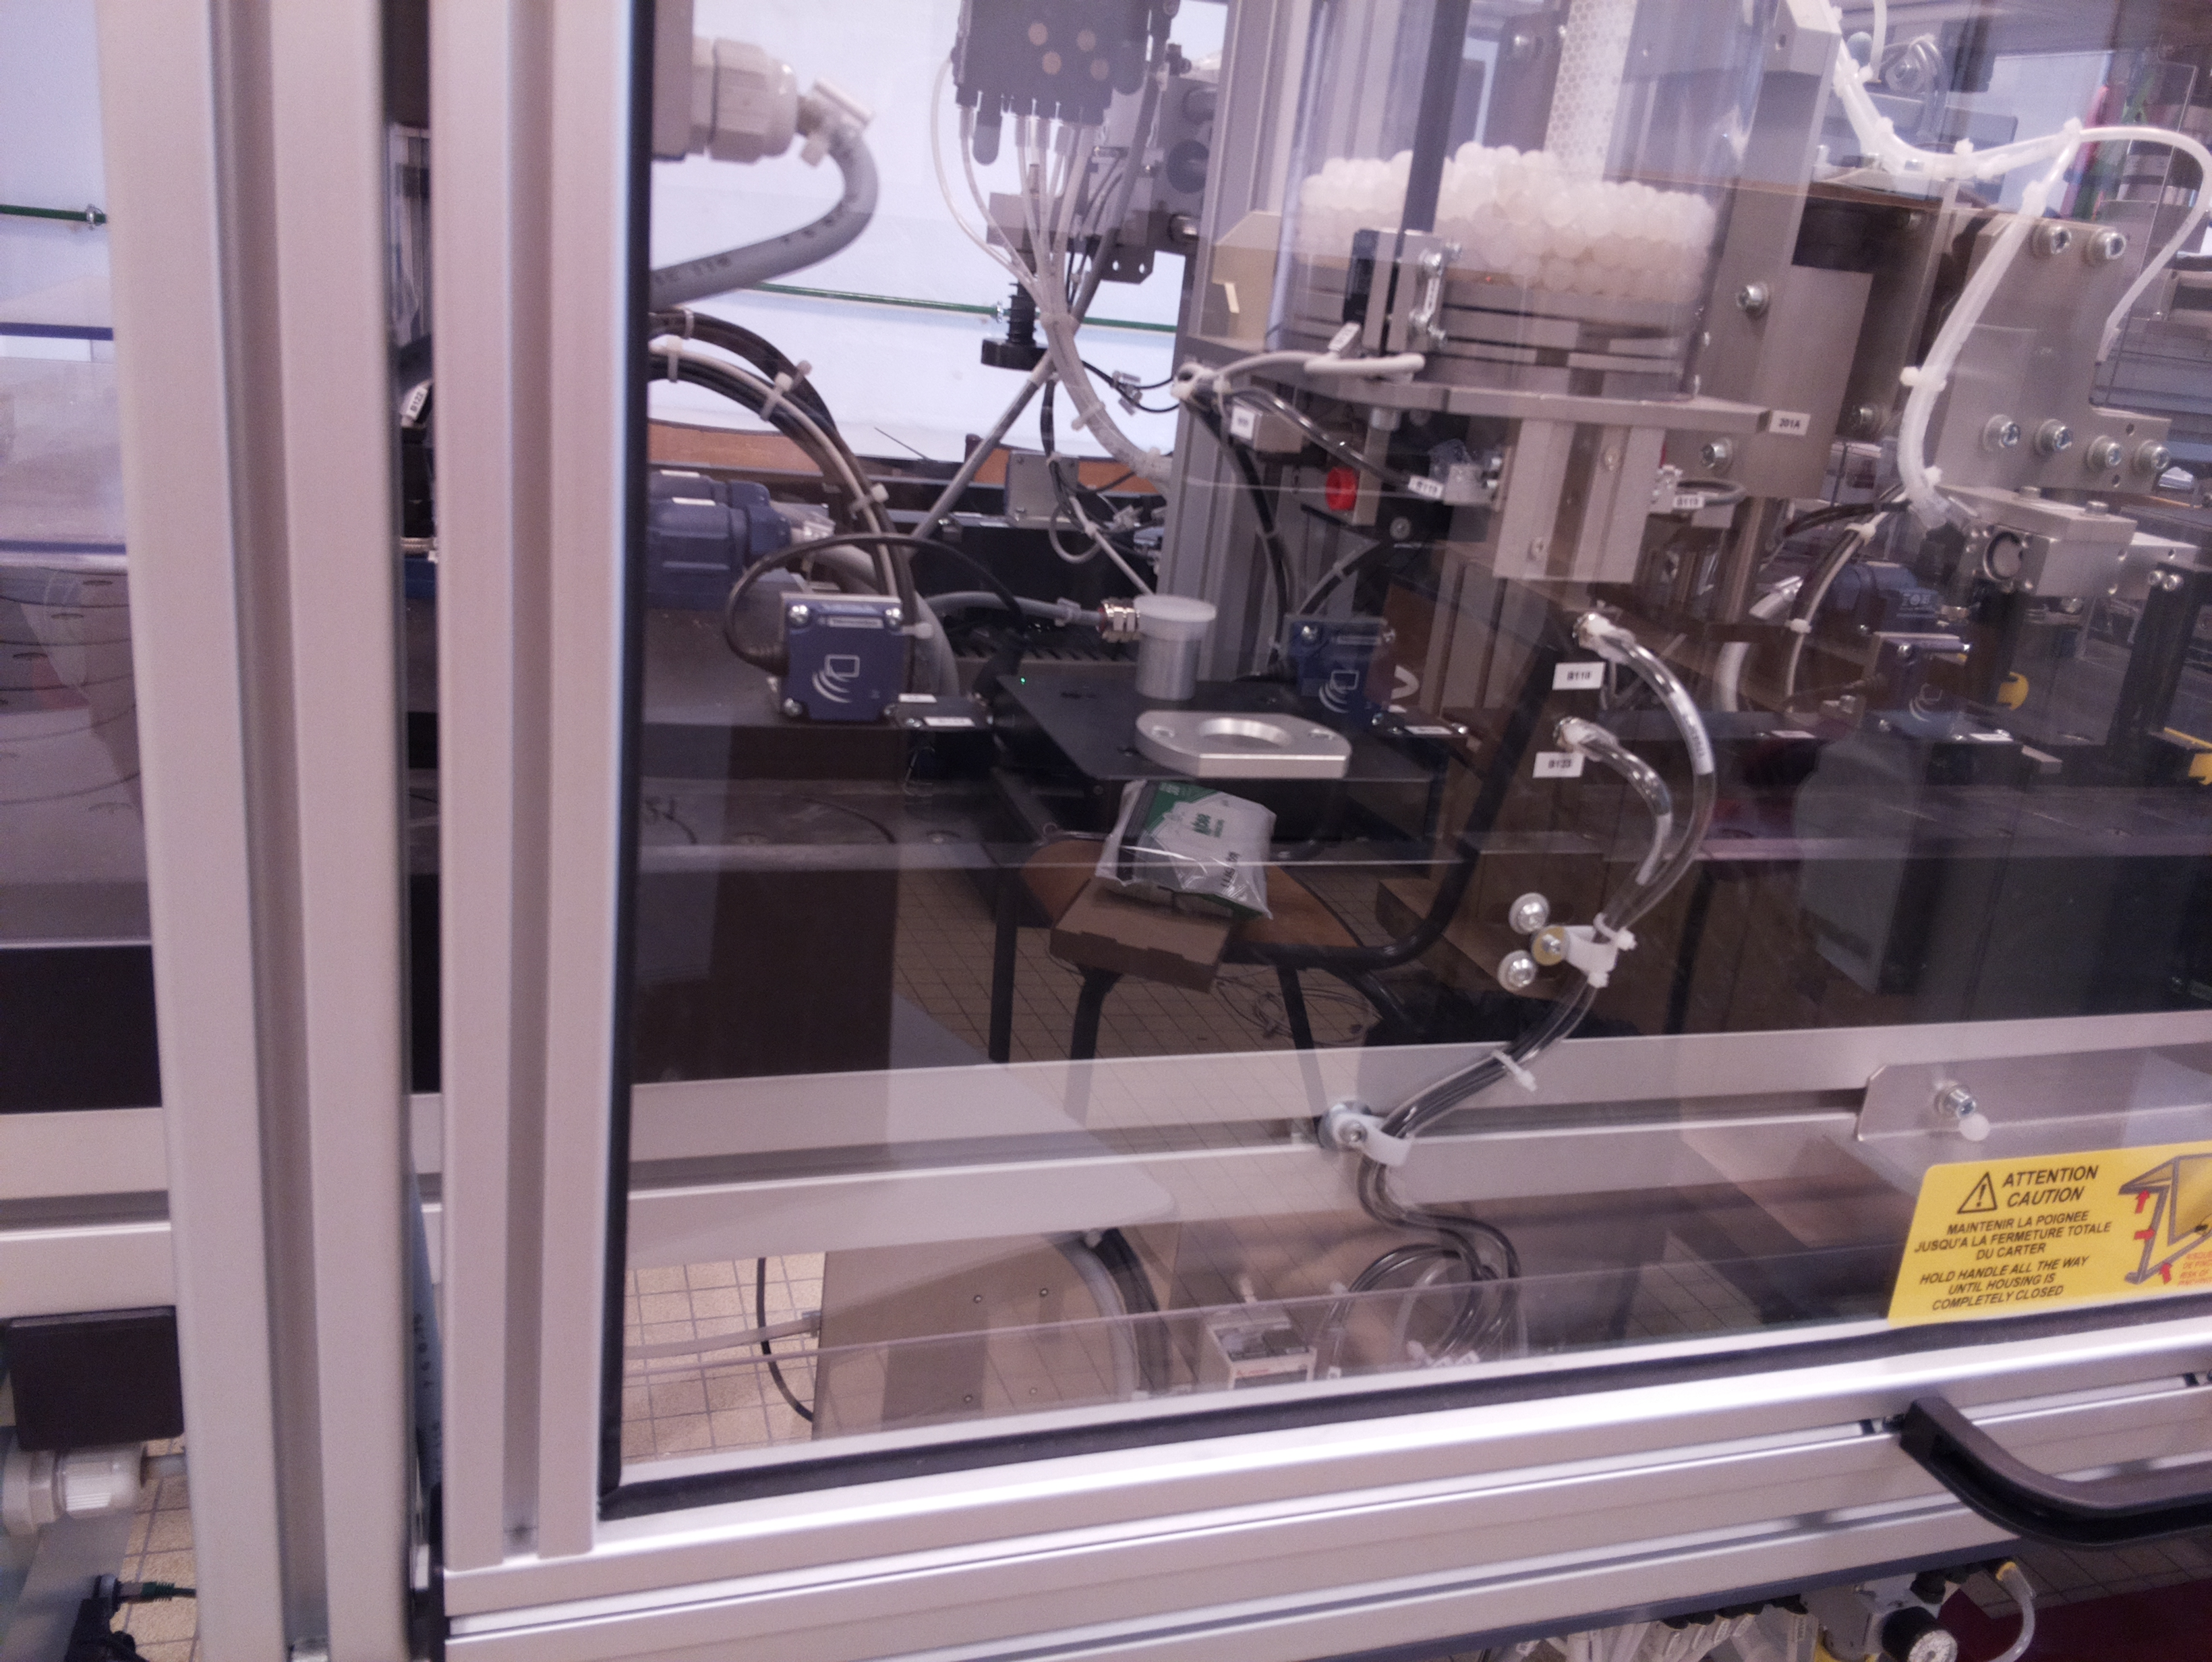
\includegraphics[width=0.8\textwidth]{image/exIA.png}}
        	\end{frame}
        	\caption{\label{fig:exIA}Exemple d'image : Anomalie Bouchon}
        \end{figure}
        
        \begin{figure}[H]
            \centering
        	\begin{frame}{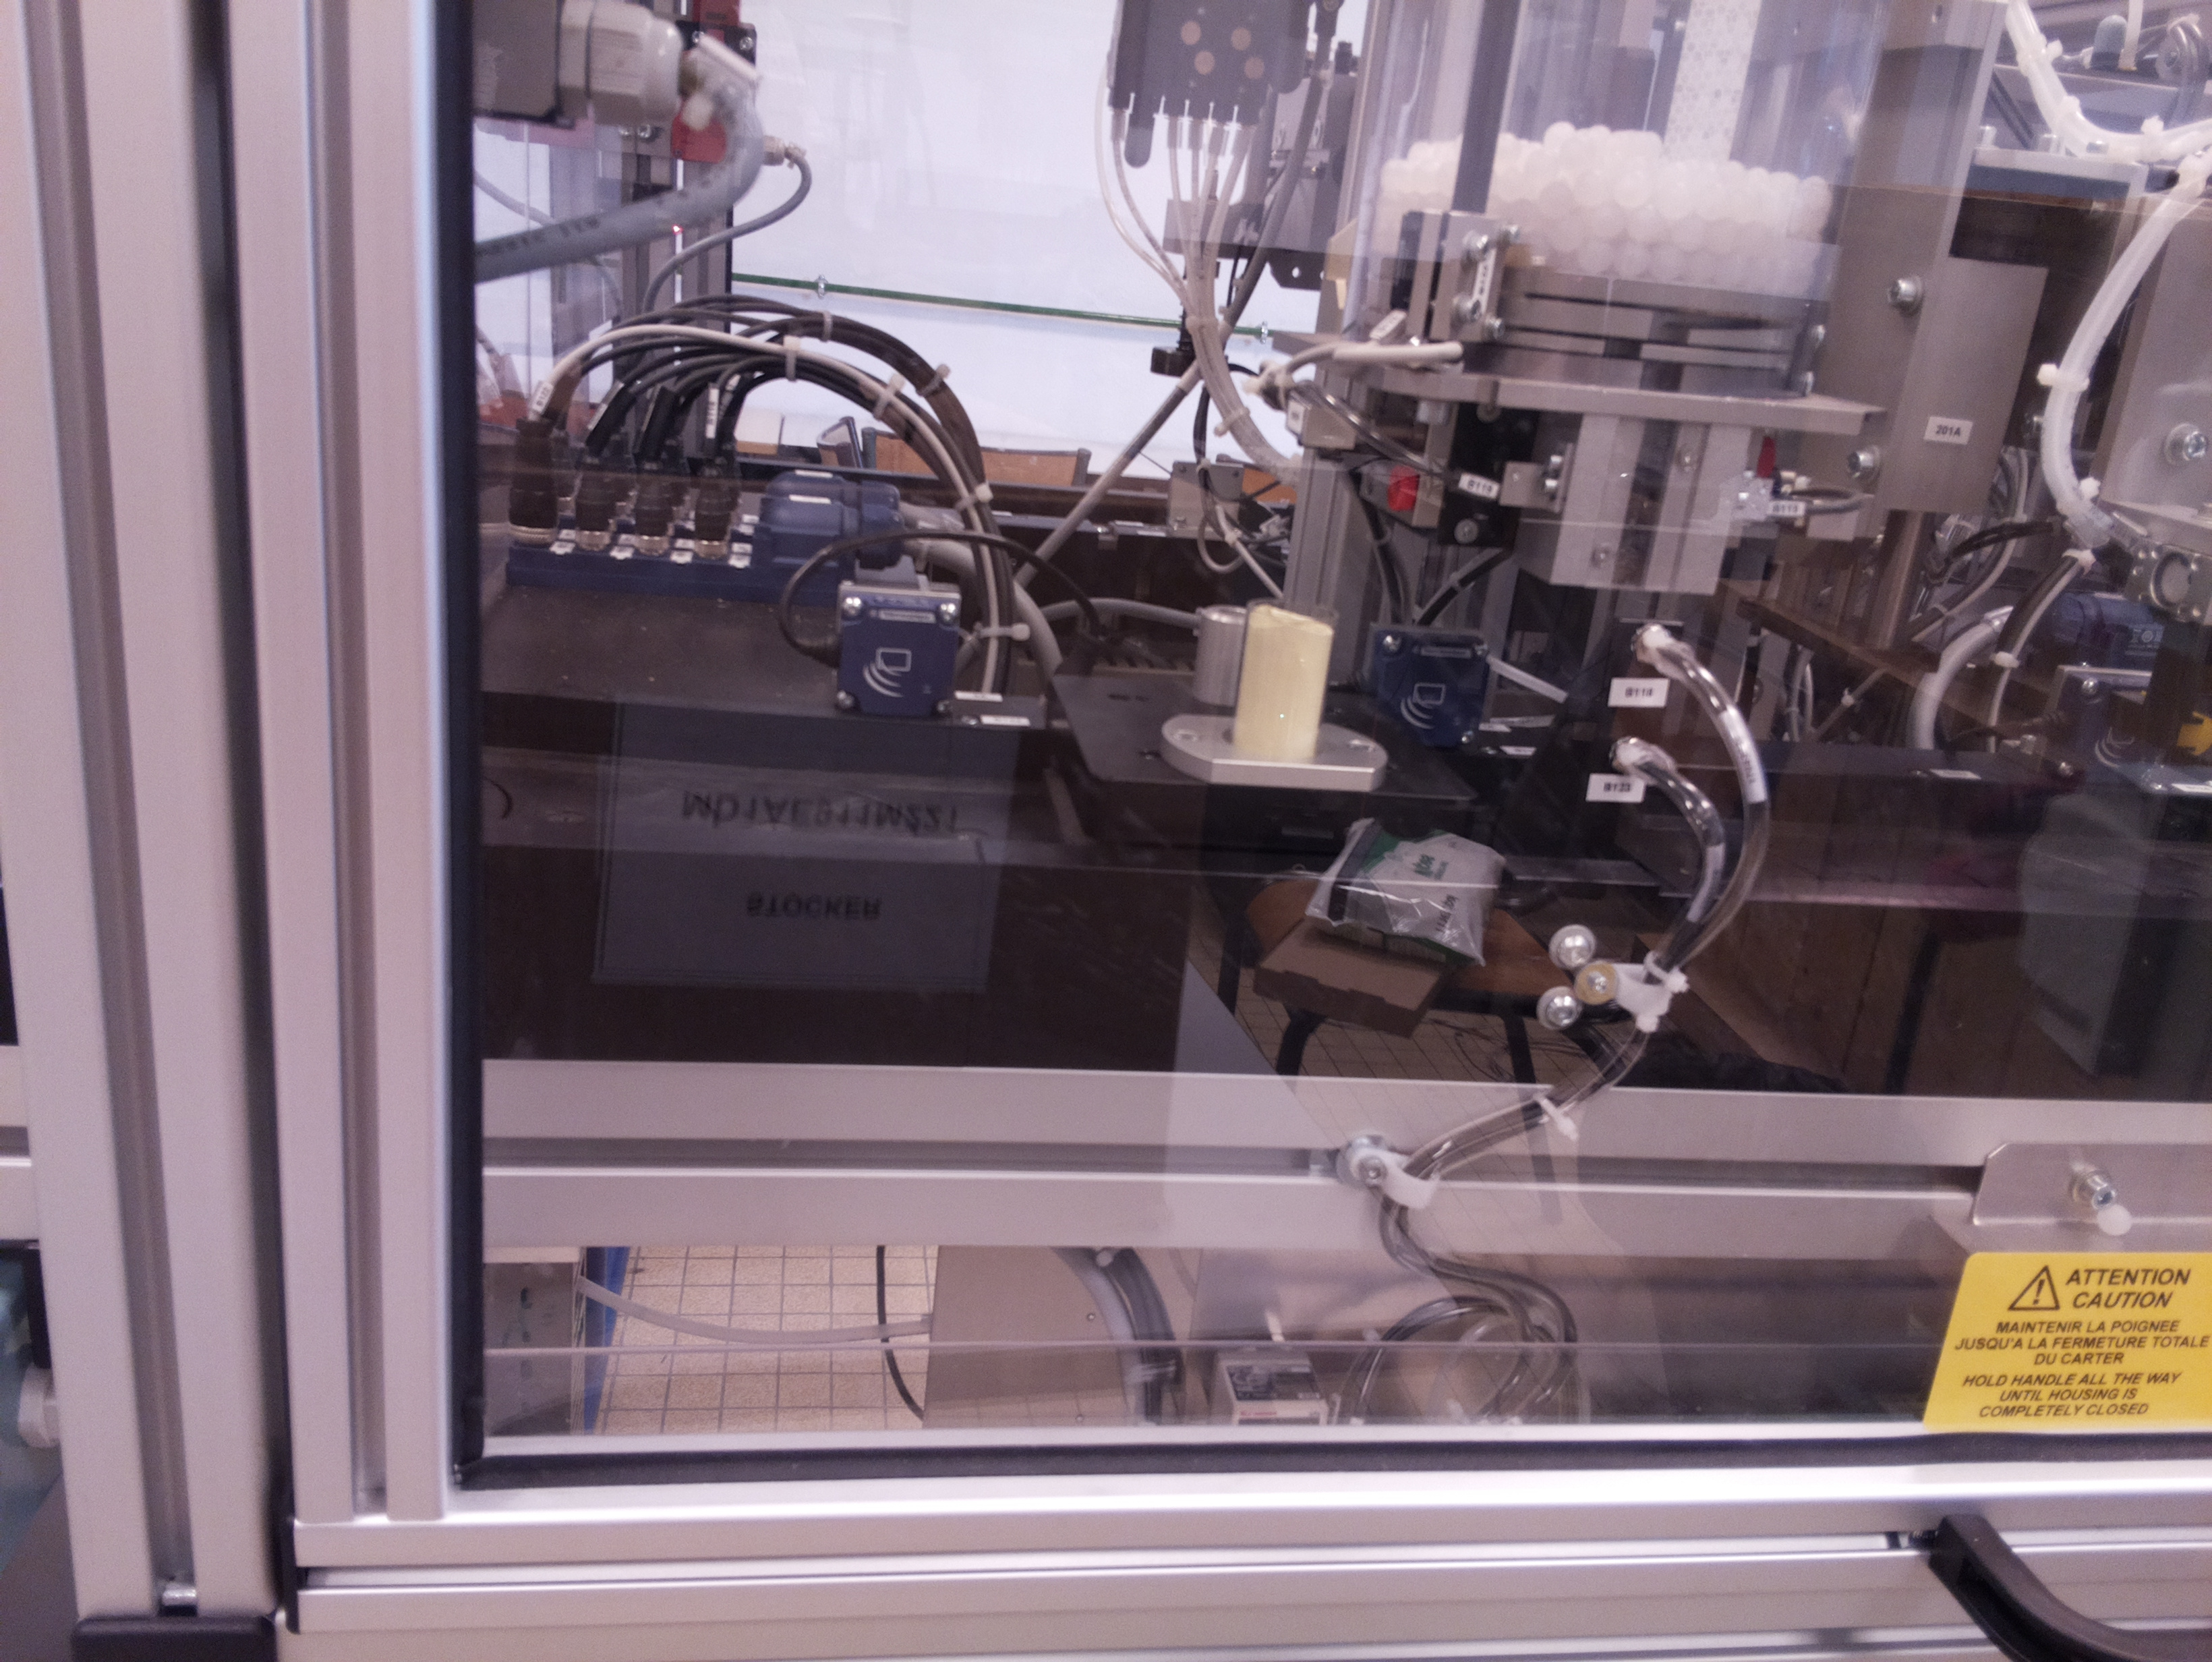
\includegraphics[width=0.8\textwidth]{image/tubeColor.png}}
        	\end{frame}
        	\caption{\label{fig:tubeColor}Exemple d'image : Anomalie Tube coloré}
        \end{figure}
        
    \subsubsection{IA : Labellisation des images}
        \paragraph*{}
        Une fois le dataset fait, il est nécessaire de labelliser les images. C'est-à-dire de renseigner les objets que l'on veut mettre en évidence sur l'image. Dans mon cas, les deux objets qui étaient à mettre en évidence étaient le tube sur la palette et le bouchon sur la palette.
        
        \paragraph*{}
        Afin de labelliser ce dataset, soit 75 images, j'ai utilisé un logiciel libre de droit, gratuit et écrit en python qui se nomme \textit{labelImg}. Il est disponible sur GitHub\cite{labelImg}. L'interface permet de choisir le répertoire de travail, de sélectionner entre le réseau de neurones Yolo et PascalVOC, créer le rectangle pour indiquer où se trouve l'objet à montrer et ensuite on peut choisir la classe de l'objet dans une liste ou ajouter un objet dans cette liste. Il est très simple d'utilisation et m'a permis de labelliser les 75 images en environ 20 minutes.
        
        \begin{figure}[H]
            \centering
        	\begin{frame}{\includegraphics[width=1\textwidth]{image/uiLabelImg.png}}
        	\end{frame}
        	\caption{\label{fig:uiLabelImg}Interface graphique de labelImg}
        \end{figure}
        
        \paragraph*{}
        Le fichier créé lors de la labellisation donne juste une ligne sous la forme : \textit{classe centreX centreY largeur hauteur}, ce qui donne par exemple pour la figure \ref{fig:zidane} quelque chose comme \textit{0 0.48 0.63 0.69 0.71} avec 0 comme étant la classe Zidane. La classe est représenté par un chiffre (0, 1, ...) selon le nombre de classes dans le dataset.
        
        \begin{figure}[H]
            \centering
        	\begin{frame}{\includegraphics[width=1\textwidth]{image/exempleImgYolo.png}}
        	\end{frame}
        	\caption{\label{fig:zidane}Exemple de labellisation avec labelImg}
        \end{figure}
    
    \subsubsection{IA : YoloV5}
    \label{part:yolo}
        \paragraph{Un réseau de neurones}
            \paragraph*{}
            YoloV5 est un système de détection d'objets en temps réel basé sur le dataset COCO. Il est très simple à comprendre et à utiliser, et permet d'avoir des résultats très rapidement pour un dataset donné. Il existe de nombreux tutoriels et exemples sur le net sur lesquels il est possible de s'appuyer afin de démarrer au mieux. Une fois qu'un modèle est entraîné, il est possible de détecter les objets sur une vidéo en temps réel. C'est une des raisons pour lesquelles il a été choisi à la place d'autres réseaux existants.
        
        \paragraph{Utilisation de Yolo}
            \paragraph*{}
            Une fois le dataset labellisé, il est nécessaire de mettre en ordre les fichiers afin que Yolo puisse apprendre. Il faut donc créer des répertoires afin de séparer les images et les labels (répertoires images/ et labels/) puis de mettre des sous dossiers pour les entrainements (train), validation et tests. Une fois ceci fait, dans le dossier de Yolo, il est nécessaire de créer un fichier YAML (\textit{Yet Another Markup Language}) qui contiendra les chemins d'accès aux dossiers précédents ainsi que les noms et le nombre de classes.
            
            Nous avons donc à présent un dossier labels et un dossier images, chacun contenant des sous-dossiers avec minimum un dossier d'entrainement et de validation (pouvant être le même que l'entrainement) et facultativement un dossier de test. Et les images et labels rangés dans les dossiers correspondants et rangés de manière aléatoire. J'avais 75 images donc 25 bouchons, 25 tubes et 25 tubes colorés; je les ai donc séparé en 17 bouchons, tube et tube coloré en entrainement (51 images) et le reste (24 images) en tests. Le dossier de validation est le même que l'entrainement.

            
        \paragraph{Apprentissage}
            \paragraph*{}
            A présent, pour l'apprentissage du modèle par le réseau de neurones, il est nécessaire tout d'abord de choisir le type de modèle. Il y a 4 modèles disponibles : le S, M, L et X.
            
            J'ai éliminé d'office le modèle S car il donnait de résultats trop médiocre bien qu'il soit plus rapide.
            Le modèle X était le meilleur mais avec une différence très petite par rapport au modèle L pour un temps d'exécution 60\% plus lent. Le choix se posait donc entre le modèle L et le modèle M, mais je me suis orienté vers le modèle L car il donnait de meilleurs résultats que le M pour une différence de temps minime.
            
            \begin{figure}[H]
                \centering
            	\begin{frame}{\includegraphics[width=1\textwidth]{image/modeleSpeedYolo.png}}
            	\end{frame}
            	\caption{\label{fig:compModeleYolo}Comparaison des modèles disponible}
            \end{figure}
            
            \paragraph*{}
            Comme il est possible de voir sur la figure \ref{fig:modeleYolo}, les valeurs veulent dire que pour le modèle S pour l'exécution et l'apprentissage du dataset COCO, il fallait 14MB en float point 16 (FP16) de mémoire, 2.0ms d'exécution sur une carte graphique Nvidia Tesla V100 en moyenne sur 5000 images et enfin, 37.2mAP (Mean Average Precision) qui est calculé en prenant la moyenne des moyennes des précisions sur toutes les classes du dataset COCO.
            
            \begin{figure}[H]
                \centering
            	\begin{frame}{\includegraphics[width=1\textwidth]{image/yolov5.png}}
            	\end{frame}
            	\caption{\label{fig:modeleYolo}Modèles disponibles pour YoloV5}
            \end{figure}
            
            \paragraph*{}
            Enfin, l'apprentissage par le réseau de neurones du dataset se fait via la commande : \texttt{python train.py --img 640 --batch 1 --epochs 100 --data plateforme.yaml --weights yolov5l.pt --cache --nosave}.
            
            \begin{itemize}
                \item img : permet de déterminer la taille des images, plus le chiffre est grand et plus le temps d'apprentissage sera élevé
                \item batch : le nombre d'images que le réseau de neurones prend à chaque propagation dans le réseau
                \item epochs : le nombre d'apprentissage. Pour les images et vidéos ce chiffre doit être grand (supérieur à 100, parfois même conseillé à 500/1000 si besoin)
                \item data : le fichier d'accès au dataset en format YAML
                \item weights : le modèle choisi
            \end{itemize}
            
        \paragraph{Résultats}
            \paragraph*{}
            La commande d'apprentissage mise dans la sous-partie précédente a mis environ 3h30 à s'exécuter avec 1 batch et 100 epochs sur 51 images de taille 640.
            
            \paragraph*{}
            A la fin de l'apprentissage, j'ai ainsi obtenu la matrice de confusion (voir figure \ref{fig:matrConfu}) ainsi que des images prédites (voir figure \ref{fig:pred0}) par l'algorithme.
            
            On voit sur la figure \ref{fig:matrConfu} que l'algorithme apprend parfaitement les bouchons et les tubes, il détecte à 100\% les images du dataset. La valeur du background FP est un élément de l'arrière plan d'une image qui a été classifié comme un tube lors de l'apprentissage. Il est impossible de voir les images incriminées pour plus de détails. Autrement, les images prédites sont très bonnes que ce soit sur les bouchons et les tubes, la prédiction est parfaite sur les images de tests que j'ai.
            
            \begin{figure}[H]
                \centering
            	\begin{frame}{\includegraphics[width=1\textwidth]{image/matriceConfusion.png}}
            	\end{frame}
            	\caption{\label{fig:matrConfu}Matrice de confusion}
            \end{figure}
            
            \begin{figure}[H]
                \centering
            	\begin{frame}{\includegraphics[width=0.9\textwidth]{image/pred0.png}}
            	\end{frame}
            	\caption{\label{fig:pred0}Exemple de prédiction faite par l'apprentissage}
            \end{figure}
        
    
    \subsubsection{Conclusion partielle}
        \paragraph*{}
        L'objectif de cette partie était l'apprentissage d'un dataset fait à partir d'anomalies possibles sur la plateforme. L'apprentissage devait se faire par un réseau de neurones qui pouvait ensuite être intégré et embarqué sur le \rpi ~afin qu'il reconnaisse une anomalie ou non si un capteur de la plateforme détecte un problème.
        
        J'ai, ainsi, grâce au logiciel \textit{labelImg} et au réseau de neurones Yolo, pu réaliser cette étape. Les résultats sont excellents et peuvent à présent être utilissé pour intégrer le réseau généré sur le drone et le \rpi ~afin que le drone puisse intervenir automatiquement en cas de panne sur la plateforme. Bien sûr, pour le moment, il est capable de détecter seulement la présence ou non d'un tube et d'un bouchon sur la palette; mais la base est présente et peut être utilisée pour aller plus loin sur les anomalies et les pannes possibles sur la plateforme entière car je me suis concentré sur la partie gauche de la plateforme (l'autre module étant en panne pour le moment).